\renewcommand*{\maketitle}{
    \begin{titlepage}
        \newgeometry{margin = 0in}
        \parindent=0pt
        % 注意这里使用了一张图片,封面使用的图片放到 config文件夹下
        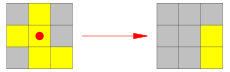
\includegraphics[width=\linewidth]{1.png}
        \vfill
        \begin{center}
            \parbox{0.618\textwidth}{
                \hfill {\bfseries \Huge \thetitle} \\[0.6pt]
                \rule{0.618\textwidth}{4pt}
            }
        \end{center}
        \vfill
        \begin{center}
            \parbox{0.618\textwidth}{
                \hfill\Large
                \begin{tabular}{r|}
                    作者:\theauthor \\
                    时间:\thedate   \\
                \end{tabular}
            }
        \end{center}
        \vfill
        \begin{center}
            \parbox[t]{0.7\textwidth}{\centering  }
        \end{center}
        \vfill
    \end{titlepage}
    \restoregeometry
    \thispagestyle{empty}
}

% 修改 名称 作者 时间
\title{自用\rm{\LaTeX}书籍模版}
\author{名字}
\date{\today}
\thispagestyle{empty}
\maketitle

\thispagestyle{empty}
\begin{center}\Huge\textbf{前言}\end{center}
前言前言前言前言前言前言前言前言前言前言前言
前言前言前言前言前言前言前言前言前言前言前言
\begin{flushright}
    \begin{tabular}{c}
        \today \\ 签名
    \end{tabular}
\end{flushright}

\newpage
\setcounter{page}{1}
\pagestyle{plain}
\pagenumbering{Roman}
\tableofcontents

\newpage
\pagestyle{plain}
\setcounter{page}{1}
\pagenumbering{arabic}